\documentclass[aspectratio=169,xcolor=table]{beamer}
\usepackage[utf8]{inputenc}
\usepackage[T1,T5]{fontenc}
\usepackage{amsmath,booktabs,array,graphicx,pifont,tikz}
\usetikzlibrary{arrows.meta,calc,positioning,fit,backgrounds}

\definecolor{Primary}{HTML}{111B88}
\definecolor{Secondary}{HTML}{101659}
\definecolor{Accent}{HTML}{F2A900}
\definecolor{SoftBlue}{HTML}{EAF2F8}
\definecolor{SoftGray}{HTML}{F3F5F7}
\definecolor{TextGray}{HTML}{4D5966}
\definecolor{RiskRed}{HTML}{A23B3B}
\definecolor{GoodGreen}{HTML}{26734D}
\definecolor{Violet}{HTML}{6D28D9}
\mode<presentation>{\usetheme{Madrid}\usecolortheme{default}\setbeamertemplate{navigation symbols}{}}
\setbeamercolor{structure}{fg=Primary}
\setbeamercolor{frametitle}{fg=white,bg=Primary}
\setbeamercolor{title}{fg=white,bg=Primary}
\setbeamercolor{block title}{fg=white,bg=Primary}
\setbeamercolor{block body}{fg=black,bg=SoftBlue}
\setbeamercolor{block title alerted}{fg=white,bg=Accent!85!black}
\setbeamercolor{block body alerted}{fg=black,bg=Accent!12}
\setbeamercolor{section in head/foot}{fg=white,bg=Primary}
\setbeamercolor{author in head/foot}{fg=white,bg=Secondary}
\setbeamercolor{date in head/foot}{fg=white,bg=Primary}
\setbeamerfont{section in head/foot}{size=\tiny,series=\bfseries}
\setbeamerfont{author in head/foot}{size=\scriptsize}
\setbeamerfont{date in head/foot}{size=\scriptsize,series=\bfseries}
\setbeamerfont{frametitle}{series=\bfseries}
\setbeamerfont{title}{series=\bfseries}
\newcommand{\decklabel}{Scorer bias word 16/10/2026}
\setbeamertemplate{itemize item}{\color{Secondary}$\blacktriangleright$}
\setbeamertemplate{itemize subitem}{\color{Accent}$\bullet$}
\setbeamertemplate{headline}{\leavevmode\begin{beamercolorbox}[wd=\paperwidth,ht=2.7ex,dp=1.1ex,leftskip=.35cm,rightskip=.35cm]{section in head/foot}\insertsectionnavigationhorizontal{\dimexpr\paperwidth-.70cm\relax}{}{}\end{beamercolorbox}}
\setbeamertemplate{footline}{\leavevmode\hbox{\begin{beamercolorbox}[wd=.55\paperwidth,ht=2.6ex,dp=1ex,leftskip=.35cm,rightskip=.20cm]{section in head/foot}\usebeamerfont{section in head/foot}\insertsectionhead\end{beamercolorbox}\begin{beamercolorbox}[wd=.27\paperwidth,ht=2.6ex,dp=1ex,center]{author in head/foot}\usebeamerfont{author in head/foot}\decklabel\end{beamercolorbox}\begin{beamercolorbox}[wd=.18\paperwidth,ht=2.6ex,dp=1ex,rightskip=.35cm plus1fil]{date in head/foot}\usebeamerfont{date in head/foot}\hfill\insertframenumber\,/\,\inserttotalframenumber\end{beamercolorbox}}}

\newcommand{\hi}[1]{\textcolor{Primary}{\textbf{#1}}}
\newcommand{\bad}[1]{\textcolor{RiskRed}{\textbf{#1}}}
\newcommand{\good}[1]{\textcolor{GoodGreen}{\textbf{#1}}}
\newcommand{\src}[1]{{\tiny\color{TextGray}[Nguồn: #1]}}
\newcommand{\cmark}{\textcolor{GoodGreen}{\ding{51}}}
\newcommand{\xmark}{\textcolor{RiskRed}{\ding{55}}}
\newcommand{\pmark}{\textcolor{Accent!85!black}{\ding{108}}}
\tikzset{
  box/.style={draw=Primary,fill=SoftBlue,rounded corners=2pt,align=center,font=\small,minimum height=0.9cm},
  lgbox/.style={draw=Accent!85!black,fill=Accent!13,rounded corners=2pt,align=center,font=\small,minimum height=0.9cm},
  nbox/.style={draw=TextGray,fill=SoftGray,rounded corners=2pt,align=center,font=\small,minimum height=0.9cm},
  vbox/.style={draw=Violet,fill=Violet!10,rounded corners=2pt,align=center,font=\small,minimum height=0.9cm},
  outbox/.style={draw=GoodGreen,fill=GoodGreen!10,rounded corners=2pt,align=center,font=\small\bfseries,minimum height=0.9cm},
  arr/.style={-{Latex[length=2mm]},thick,draw=TextGray},
}

\title{Scorer chọn bias word theo audio\\Tái hiện Hou25 + 2 biến thể}
\subtitle{Báo cáo A--Z: data, kiến trúc, train, inference, kết quả thử}
\author{Nhóm Contextual ASR}
\institute{}
\date{16/10/2026}
\setbeamertemplate{title page}{\begin{centering}\vspace*{0.10cm}
\includegraphics[height=1.08cm]{imgs/logo.png}\par\vspace{0.32cm}\begin{beamercolorbox}[sep=0.50em,center,rounded=true]{title}\usebeamerfont{title}\inserttitle\par\vspace{0.14cm}{\small\insertsubtitle\par}\end{beamercolorbox}\vspace{0.42cm}{\usebeamerfont{author}\insertauthor\par}\vspace{0.10cm}{\usebeamerfont{institute}\insertinstitute\par}\vfill{\usebeamerfont{date}\insertdate\par}\end{centering}}

\begin{document}
\begin{frame}[plain]\titlepage\end{frame}

% =====================================================================
\section{Tóm tắt}
\begin{frame}{Tóm tắt: đã làm gì, đang ở đâu}
\begin{center}
\begin{tikzpicture}[node distance=0.3cm]
\node[outbox,minimum width=2.6cm,text width=2.4cm,minimum height=1.5cm] (a) {1. Data\\\footnotesize\cmark\ 209.604 từ\\TTS + encode};
\node[outbox,right=of a,minimum width=2.6cm,text width=2.4cm,minimum height=1.5cm] (b) {2. Kiến trúc\\\footnotesize\cmark\ 3 model\\đã kiểm code};
\node[lgbox,right=of b,minimum width=2.6cm,text width=2.4cm,minimum height=1.5cm] (c) {3. Train\\\footnotesize\pmark\ mới thử\\800 câu, 1 epoch};
\node[outbox,right=of c,minimum width=2.6cm,text width=2.4cm,minimum height=1.5cm] (d) {4. Inference\\\footnotesize\cmark\ 1 tầng + cascade};
\node[nbox,right=of d,minimum width=2.6cm,text width=2.4cm,minimum height=1.5cm] (e) {5. B-WER\\\footnotesize\xmark\ chưa có};
\draw[arr] (a)--(b); \draw[arr] (b)--(c); \draw[arr] (c)--(d); \draw[arr] (d)--(e);
\end{tikzpicture}
\end{center}
\vspace{0.2cm}
\begin{beamercolorbox}[sep=0.6em,rounded=true]{block body alerted}
\small\textbf{Kết luận trước:}
\begin{itemize}\itemsep2pt
\item Đã dựng xong \textbf{toàn bộ pipeline} tái hiện Hou25 (paper không có code), thêm \hi{nocross} (ablation) và \hi{maxsim} (model rẻ, làm \textbf{cascade} rút gọn list).
\item Train thử: cả 3 model \good{đã học được} (Recall@10 khoảng 29--36\% so với $\sim$10\% ngẫu nhiên), nhưng \bad{chưa đủ để so kiến trúc}.
\item Chưa có B-WER. Feature 21\,GB đã \bad{bị xoá khi dọn server} $\rightarrow$ cần $\sim$2\,giờ dựng lại.
\end{itemize}
\end{beamercolorbox}
\end{frame}

% =====================================================================
\section{Vì sao cần scorer}
\begin{frame}{Vì sao cần chọn lọc list: list càng dài, bias càng mất tác dụng}
\begin{columns}[T]
\begin{column}{0.56\textwidth}
\centering
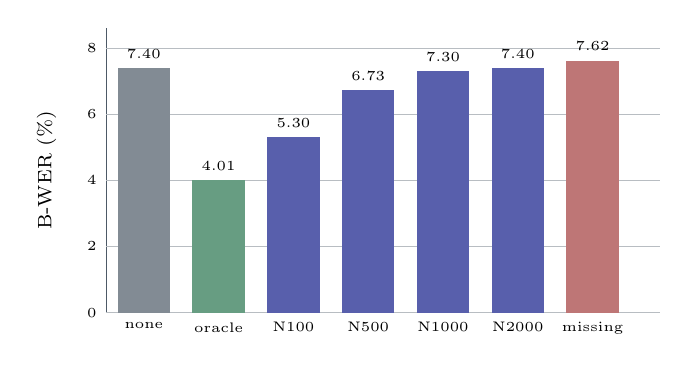
\begin{tikzpicture}[x=0.95cm,y=0.42cm]
\draw[TextGray] (0,0)--(7.4,0);
\draw[TextGray] (0,0)--(0,8.6);
\foreach \yy in {0,2,4,6,8} {\draw[TextGray!40] (0,\yy)--(7.4,\yy); \node[left,font=\tiny] at (0,\yy) {\yy};}
\foreach \xx/\vv/\ll/\cc in {0.5/7.40/none/TextGray, 1.5/4.01/oracle/GoodGreen, 2.5/5.30/N100/Primary, 3.5/6.73/N500/Primary, 4.5/7.30/N1000/Primary, 5.5/7.40/N2000/Primary, 6.5/7.62/missing/RiskRed}
{\fill[\cc!70] (\xx-0.35,0) rectangle (\xx+0.35,\vv); \node[above,font=\tiny] at (\xx,\vv) {\vv}; \node[below,font=\tiny] at (\xx,0) {\ll};}
\node[rotate=90,font=\scriptsize] at (-0.8,4.3) {B-WER (\%)};
\end{tikzpicture}\\
{\scriptsize Qwen3-ASR-1.7B frozen, LibriSpeech test-clean, 2620 câu, wnorm}
\end{column}
\begin{column}{0.42\textwidth}
\small
\begin{itemize}\itemsep4pt
\item Oracle (chỉ từ đúng): B-WER \good{7.40 $\rightarrow$ 4.01}.
\item Thêm 2000 từ nhiễu: \bad{7.40}, mất hết lợi ích.
\item List chỉ toàn từ sai: \bad{7.62}, tệ hơn không dùng.
\end{itemize}
\vspace{0.2cm}
\begin{beamercolorbox}[sep=0.5em,rounded=true]{block body}
\footnotesize\textbf{Ý tưởng scorer:} trước khi đưa list vào ASR, \textbf{chấm từng từ theo audio}, giữ top-50 $\rightarrow$ kéo N=2000 về gần oracle.
\end{beamercolorbox}
\vspace{0.1cm}
\src{bench/results.md, chạy 02--03/10}
\end{column}
\end{columns}
\end{frame}

\begin{frame}{Hou25 (Interspeech 2025): so \emph{âm thanh} với \emph{âm thanh}}
\begin{center}
\begin{tikzpicture}[node distance=0.45cm]
\node[lgbox,minimum width=2.2cm] (w) {``cardamom''};
\node[nbox,right=of w,minimum width=2.0cm] (tts) {TTS};
\node[nbox,right=of tts,minimum width=2.9cm] (wa) {audio của từ};
\node[lgbox,below=0.5cm of w,minimum width=2.2cm] (sp) {câu nói};
\node[box,right=1.2cm of $(wa)!0.5!(sp-|wa)$,minimum width=2.4cm,minimum height=1.6cm] (sc) {Scorer\\\footnotesize(có train)};
\node[outbox,right=of sc,minimum width=2.4cm] (o) {điểm\\\footnotesize``có trong câu?''};
\draw[arr] (w)--(tts); \draw[arr] (tts)--(wa); \draw[arr] (wa.east)--(sc); \draw[arr] (sp.east)--(sc); \draw[arr] (sc)--(o);
\end{tikzpicture}
\end{center}
\vspace{0.15cm}
\footnotesize
\begin{columns}[T]
\begin{column}{0.5\textwidth}
\textbf{Paper báo cáo} (Whisper-turbo, B-WER test-clean):\\[2pt]
\renewcommand{\arraystretch}{1.15}
\begin{tabular}{@{}lcc@{}}
\toprule
& N=100 & N=2000\\
\midrule
Cả list vào prompt & 7.8 & 9.8\\
Scorer, top-50 & \good{5.4} & \good{5.8}\\
\bottomrule
\end{tabular}\\
\src{Hou25, Bảng 1; ``giảm hơn 40\%'' ứng với N lớn}
\end{column}
\begin{column}{0.48\textwidth}
\textbf{Vấn đề khi tái hiện:}
\begin{itemize}\itemsep2pt
\item \bad{Không có code} $\rightarrow$ phải tự viết.
\item Nhiều chi tiết \textbf{không nói}: loss, tỉ lệ negative, giọng TTS, encoder có đóng băng không\dots
\item Mỗi câu chấm N=2000 từ bằng CNN $\rightarrow$ \textbf{đắt}.
\end{itemize}
\end{column}
\end{columns}
\end{frame}

% =====================================================================
\section{Tổng quan}
\begin{frame}{Toàn cảnh hệ thống: data (chạy 1 lần) và inference}
\centering
{\small\hi{Data}: mỗi bias word được đọc bằng TTS, rồi cùng câu nói đi qua 1 encoder đóng băng}\\[2pt]
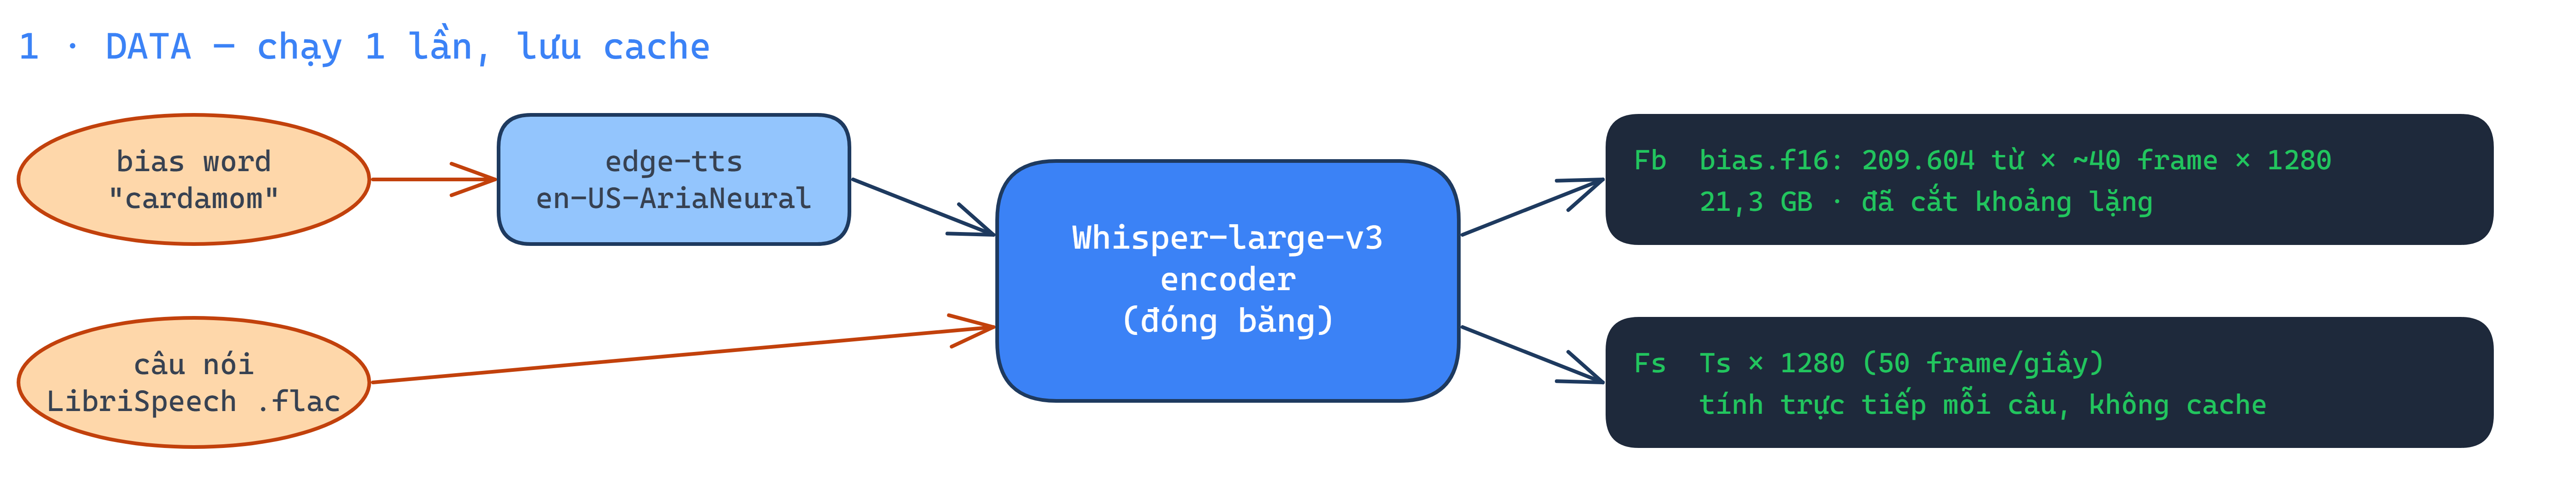
\includegraphics[width=0.86\textwidth]{imgs/arch_data.png}\\[4pt]
{\small\hi{Inference}: lọc rẻ trước, chấm kỹ sau, chỉ giữ 50 từ cho ASR}\\[2pt]
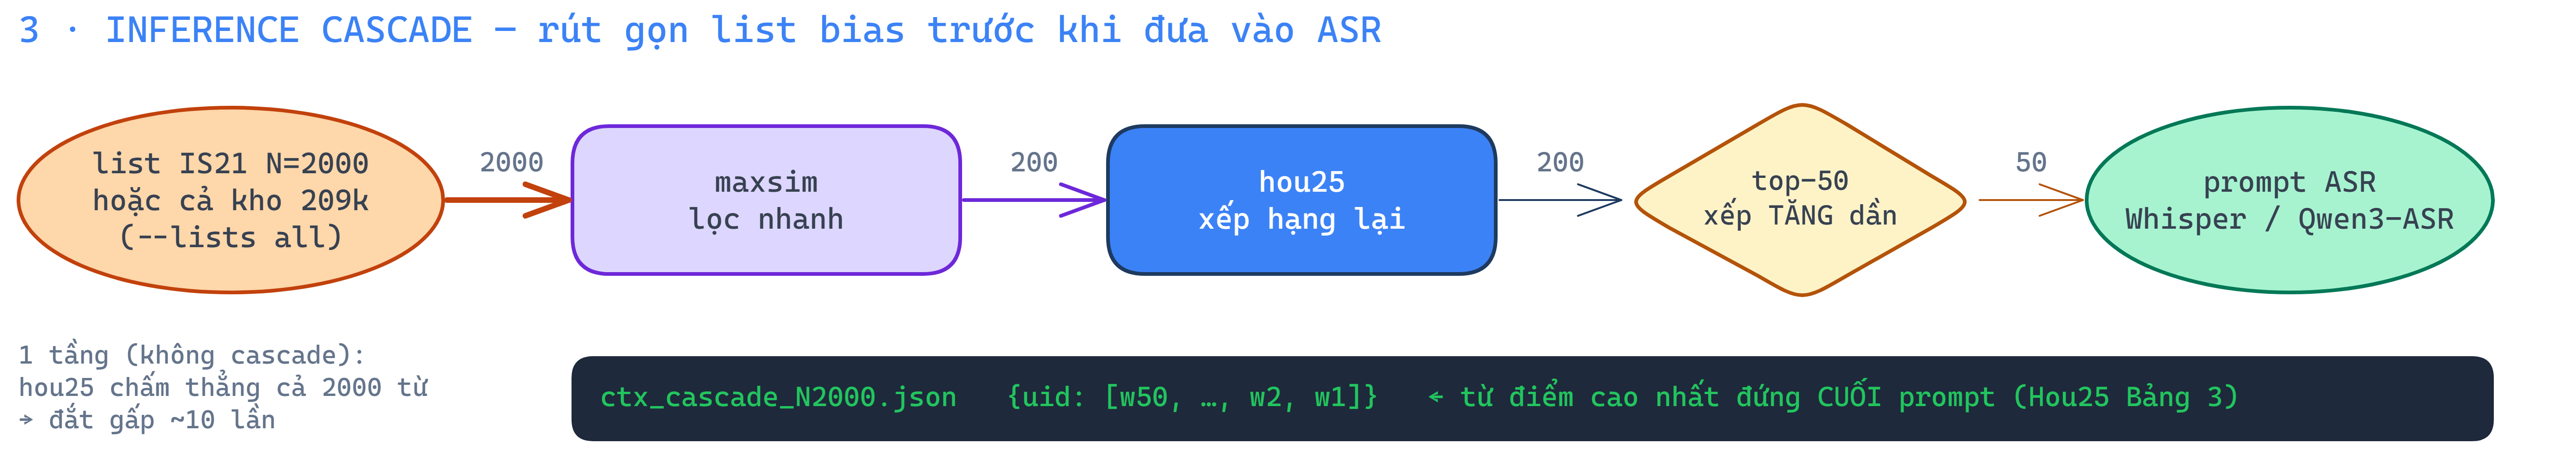
\includegraphics[width=0.86\textwidth]{imgs/arch_cascade.png}
\end{frame}

\begin{frame}{Ba kiến trúc cạnh nhau}
\centering
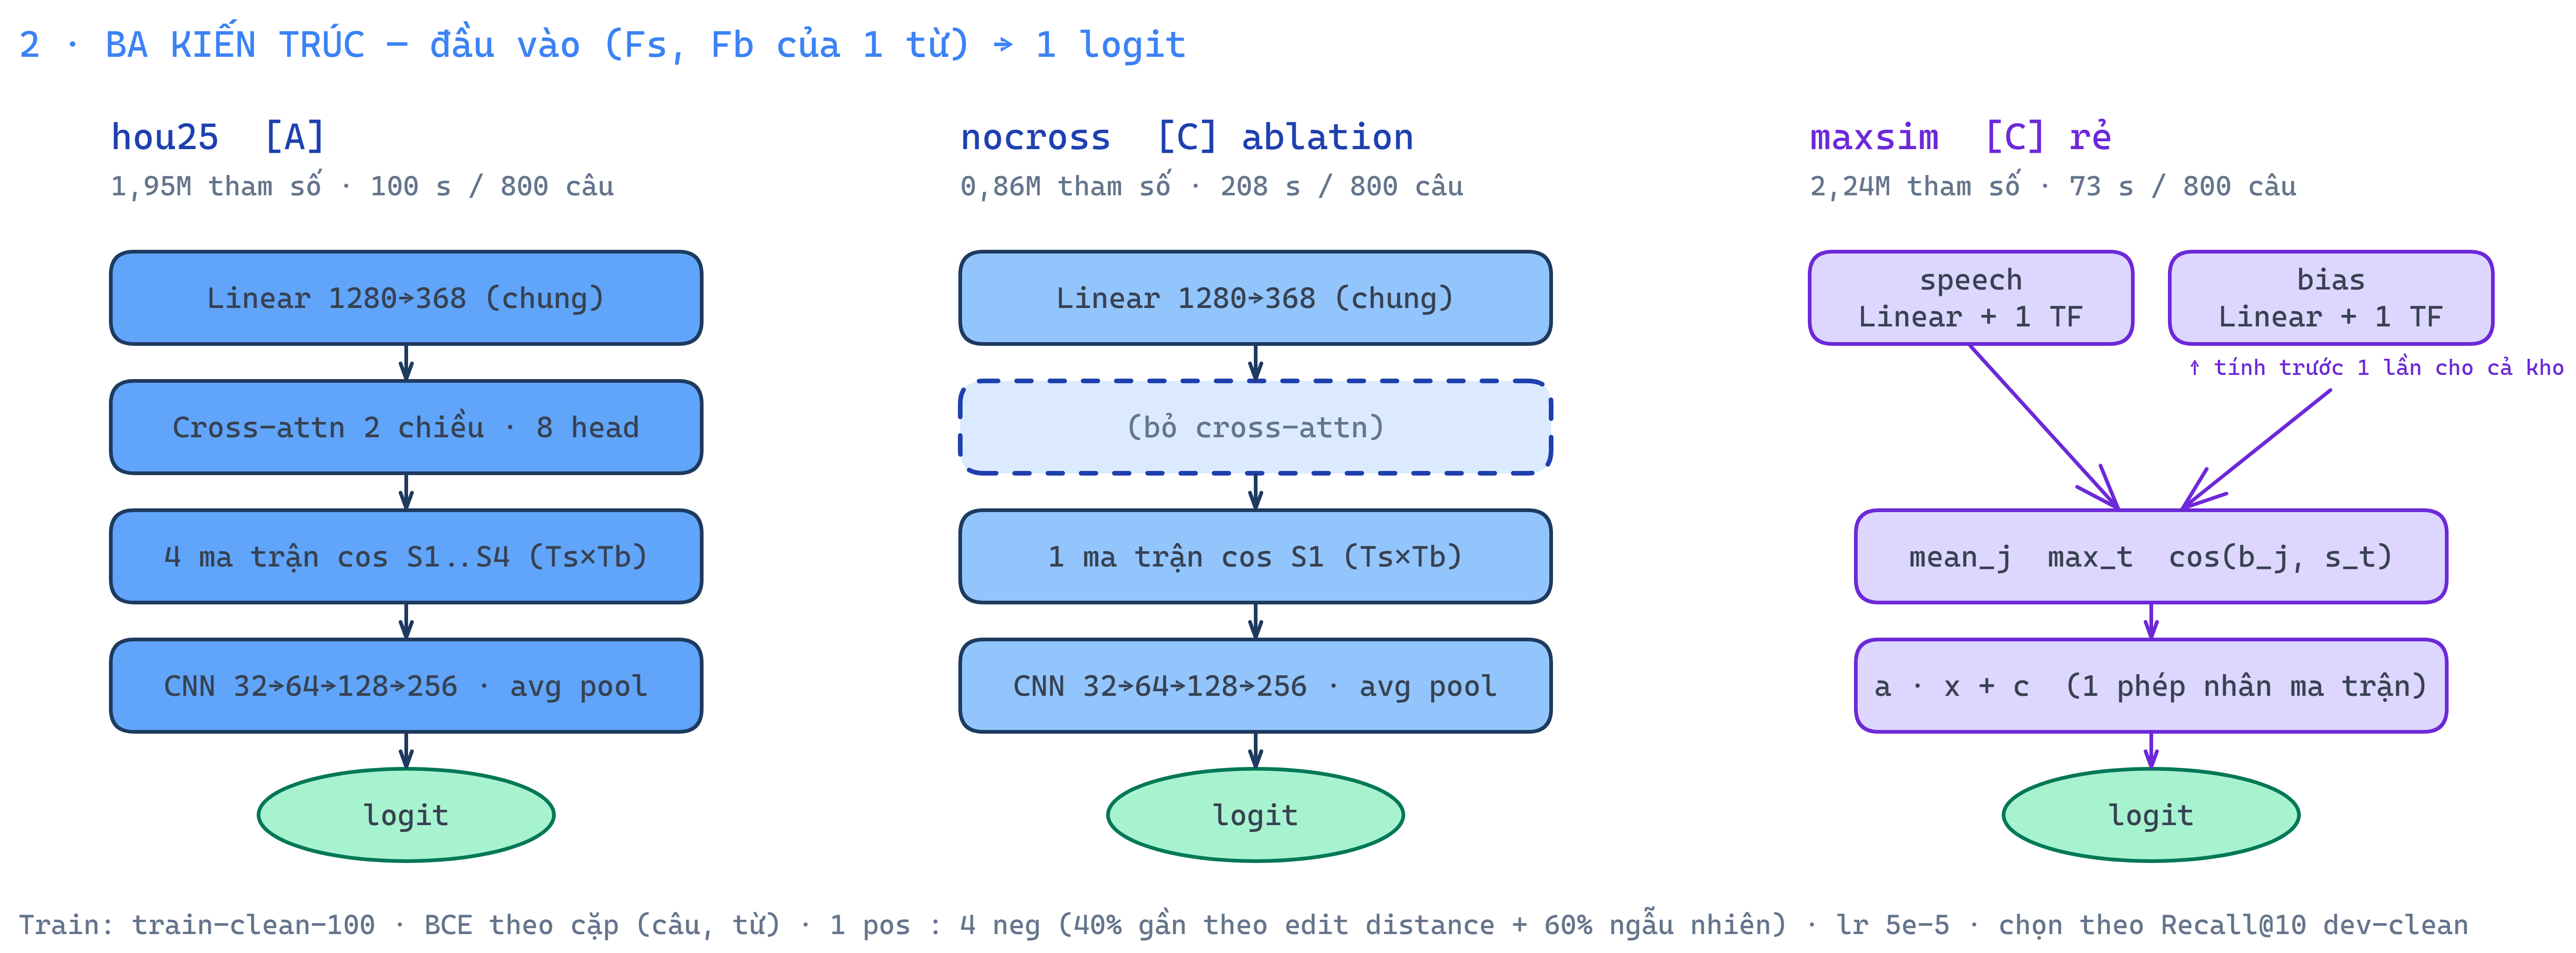
\includegraphics[width=\textwidth]{imgs/arch_models.png}
\end{frame}

\begin{frame}{Code tổ chức theo 3 phần: data $\rightarrow$ training $\rightarrow$ inference}
\begin{columns}[T]
\begin{column}{0.48\textwidth}
\footnotesize
\begin{beamercolorbox}[sep=0.5em,rounded=true]{block body}
\ttfamily\scriptsize
scorer/\\
\ \ common.py \ \ \ \ \ \textrm{\color{TextGray}encoder, kho feature}\\
\ \ models.py \ \ \ \ \ \textrm{\color{TextGray}hou25 | nocross | maxsim}\\
\ \ data/\\
\ \ \ \ build\_train.py \textrm{\color{TextGray}bước 1}\\
\ \ \ \ tts.py \ \ \ \ \ \ \ \ \textrm{\color{TextGray}bước 2}\\
\ \ \ \ encode\_bias.py \textrm{\color{TextGray}bước 3}\\
\ \ training/train.py \textrm{\color{TextGray}bước 4}\\
\ \ inference/rank.py \textrm{\color{TextGray}bước 5}\\
\ \ work/ \ \ \ \ \ \ \ \ \ \textrm{\color{TextGray}output nặng, chỉ ở server}\\
\ \ README.md, architecture.png
\end{beamercolorbox}
\end{column}
\begin{column}{0.50\textwidth}
\small
\begin{itemize}\itemsep4pt
\item Đổi kiến trúc chỉ bằng 1 cờ: \texttt{--arch hou25}.
\item Output của bước 5 là \texttt{ctx\_<tên>\_N2000.json}, \textbf{cùng định dạng} với protocol cũ $\rightarrow$ chạy thẳng \texttt{run\_whisper.py}, \texttt{run\_qwen3asr.py}.
\item Mọi lựa chọn đều gắn nhãn nguồn:\\
\hi{[A]} theo paper, \hi{[B]} thông lệ, \hi{[C]} nhóm tự thiết kế.
\end{itemize}
\end{column}
\end{columns}
\end{frame}

% =====================================================================
\section{Data}
\begin{frame}{Bước 1--3: dựng data (đã chạy xong trên 1 GPU RTX 4090)}
\begin{center}
\begin{tikzpicture}[node distance=0.35cm]
\node[nbox,minimum width=3.0cm,text width=2.9cm,minimum height=1.9cm] (a) {\textbf{1. build\_train}\\\footnotesize train-clean-100\\28.539 câu\\dev-clean 2.703 câu};
\node[nbox,right=of a,minimum width=3.0cm,text width=2.9cm,minimum height=1.9cm] (b) {\textbf{2. tts}\\\footnotesize edge-tts\\209.604 từ, \good{0 lỗi}\\$\sim$43 từ/s, 80 phút};
\node[box,right=of b,minimum width=3.0cm,text width=2.9cm,minimum height=1.9cm] (c) {\textbf{3. encode\_bias}\\\footnotesize Whisper-large-v3\\đóng băng\\$\sim$25 phút};
\node[outbox,right=of c,minimum width=3.0cm,text width=2.9cm,minimum height=1.9cm] (d) {bias.f16\\\footnotesize 8,33 triệu frame\\$\times$ 1280 chiều\\21,3 GB};
\draw[arr] (a)--(b); \draw[arr] (b)--(c); \draw[arr] (c)--(d);
\end{tikzpicture}
\end{center}
\vspace{0.1cm}
\footnotesize
\begin{columns}[T]
\begin{column}{0.5\textwidth}
\textbf{Từ cần đọc (vocab TTS)} = kho 209k từ hiếm IS21 $\cup$ từ hiếm của train/dev $\cup$ mọi từ trong list test.\\[3pt]
\textbf{Mỗi từ} $\approx$ 0,8 giây audio $\rightarrow$ trung bình \textbf{40 frame}. Đã cắt khoảng lặng đầu/cuối.
\end{column}
\begin{column}{0.48\textwidth}
\textbf{Câu nói} không lưu feature trước (sẽ tốn thêm $\sim$45\,GB): encode trực tiếp mỗi lần train.\\[3pt]
\textbf{Chỉ lưu 1 file liền} + 1 file chỉ mục \texttt{từ, offset, số frame} $\rightarrow$ đọc nhanh bằng memmap.
\end{column}
\end{columns}
\end{frame}

\begin{frame}{Một mẫu train thật: từ đúng + từ sai ``dễ nhầm''}
\small
Câu \texttt{103-1240-0006} (train-clean-100), 28 từ khác nhau, có \textbf{3 từ hiếm}:
\vspace{0.2cm}
\begin{center}
\begin{tikzpicture}[node distance=0.25cm]
\node[outbox,minimum width=2.6cm] (p1) {avonlea};
\node[outbox,below=of p1,minimum width=2.6cm] (p2) {awed};
\node[outbox,below=of p2,minimum width=2.6cm] (p3) {housekeepers};
\node[font=\footnotesize\bfseries,GoodGreen,above=0.1cm of p1] {positive (nhãn 1)};
\node[lgbox,right=1.2cm of p1,minimum width=6.2cm,font=\footnotesize] (n1) {avonley, avonne, avenge, yvonne, volley};
\node[lgbox,right=1.2cm of p2,minimum width=6.2cm,font=\footnotesize] (n2) {owed, wed, sawed, abed, jawed};
\node[lgbox,right=1.2cm of p3,minimum width=6.2cm,font=\footnotesize] (n3) {housekeeper's, housekeeping, hotelkeepers, \dots};
\node[font=\footnotesize\bfseries,Accent!70!black,above=0.1cm of n1] {negative khó: gần nhất theo edit distance};
\draw[arr] (p1)--(n1); \draw[arr] (p2)--(n2); \draw[arr] (p3)--(n3);
\end{tikzpicture}
\end{center}
\vspace{0.1cm}
\footnotesize
\begin{itemize}\itemsep2pt
\item Mỗi câu: tối đa 8 positive; negative = 4 $\times$ số positive: \textbf{40\% từ khó} (như trên) + \textbf{60\% ngẫu nhiên} trong kho 209k. \hi{[A]} tỉ lệ 40/60, \hi{[B]} tỉ lệ 1:4.
\item Không lấy làm negative những từ có mặt trong câu. Trung bình mỗi câu 3,4 từ hiếm; 26.422/28.539 câu có ít nhất 1 từ hiếm.
\end{itemize}
\end{frame}

% =====================================================================
\section{Kiến trúc}
\begin{frame}{hou25: ma trận frame $\times$ frame $\rightarrow$ CNN tìm ``vệt chéo''}
\begin{columns}[T]
\begin{column}{0.47\textwidth}
\centering
\begin{tikzpicture}[x=0.27cm,y=0.27cm]
% ma trận Ts x Tb: câu (ngang) x từ (dọc)
\foreach \xx in {0,...,17} \foreach \yy in {0,...,7} {\fill[SoftBlue] (\xx,\yy) rectangle +(0.92,0.92);}
\foreach \kk in {0,...,7} {\pgfmathtruncatemacro{\cx}{8+\kk}\pgfmathtruncatemacro{\cy}{7-\kk}\fill[Primary] (\cx,\cy) rectangle +(0.92,0.92);}
\foreach \kk in {0,...,6} {\pgfmathtruncatemacro{\cx}{8+\kk}\pgfmathtruncatemacro{\cy}{6-\kk}\fill[Primary!45] (\cx,\cy) rectangle +(0.92,0.92);\pgfmathtruncatemacro{\cz}{9+\kk}\pgfmathtruncatemacro{\cw}{7-\kk}\fill[Primary!45] (\cz,\cw) rectangle +(0.92,0.92);}
\fill[Primary!30] (2,5) rectangle +(0.92,0.92); \fill[Primary!30] (13,1) rectangle +(0.92,0.92);
\node[font=\scriptsize] at (9,-1.2) {frame của câu nói (Ts)};
\node[font=\scriptsize,rotate=90] at (-1.2,4) {frame của từ (Tb)};
\draw[Accent,very thick,rounded corners=1pt] (7.8,-0.2) rectangle (16.1,8.1);
\node[font=\scriptsize\bfseries,Accent!80!black] at (12,9.3) {đoạn câu nói chứa từ};
\end{tikzpicture}\\[2pt]
{\scriptsize Từ có trong câu $\Rightarrow$ một \textbf{đường chéo sáng}.\\Ô sáng lẻ tẻ = trùng âm ngẫu nhiên.}
\end{column}
\begin{column}{0.52\textwidth}
\footnotesize
\begin{enumerate}\itemsep3pt
\item \textbf{Linear} 1280 $\rightarrow$ 368 cho cả câu và từ \hi{[A]} (dùng chung 1 lớp \hi{[B]}).
\item \textbf{Cross-attention 2 chiều}, 8 head \hi{[A]}:\\câu ``nhìn'' từ $\rightarrow$ $F_{s\to b}$; từ ``nhìn'' câu $\rightarrow$ $F_{b\to s}$.
\item \textbf{4 ma trận cosine} $T_s\times T_b$ \hi{[A]}:\\
$S_1{=}\cos(F_s,F_b)$, $S_2{=}\cos(F_s,F_{b\to s})$,\\$S_3{=}\cos(F_{s\to b},F_b)$, $S_4{=}\cos(F_{s\to b},F_{b\to s})$.
\item Xếp 4 ma trận thành ảnh 4 kênh $\rightarrow$ \textbf{CNN} 32/64/128/256 kênh, kernel 3 \hi{[A]}.
\item \textbf{Avg pool} (chỉ trên vùng không pad \hi{[B]}) $\rightarrow$ Linear $\rightarrow$ \textbf{1 logit}.
\end{enumerate}
\vspace{2pt}
\textbf{1,95M tham số} được train; encoder Whisper đóng băng.
\end{column}
\end{columns}
\end{frame}

\begin{frame}{nocross và maxsim: hai biến thể để đo và để chạy nhanh}
\begin{columns}[T]
\begin{column}{0.40\textwidth}
\begin{beamercolorbox}[sep=0.5em,rounded=true]{block body}
\small\textbf{nocross} \hi{[C]} --- ablation\\[2pt]
\footnotesize Giống hou25 nhưng \textbf{bỏ cross-attention}, chỉ còn $S_1$ $\rightarrow$ CNN.\\[3pt]
0,86M tham số.\\[3pt]
\textbf{Trả lời:} cross-attention đóng góp bao nhiêu? Nếu nocross $\approx$ hou25 thì phần đó không đáng.
\end{beamercolorbox}
\end{column}
\begin{column}{0.58\textwidth}
\begin{beamercolorbox}[sep=0.5em,rounded=true]{block body}
\small\textbf{maxsim} \hi{[C]} --- late interaction (kiểu ColBERT)\\[2pt]
\centering
\begin{tikzpicture}[x=0.42cm,y=0.42cm]
\foreach \xx in {0,...,13} {\fill[Primary!25] (\xx,0) circle (0.17);}
\node[font=\tiny,left] at (-0.3,0) {câu nói};
\foreach \xx in {0,...,3} {\fill[Violet] (4.5+\xx*1.2,2.6) circle (0.17);}
\node[font=\tiny,left] at (4.1,2.6) {từ};
\draw[Violet,thick,->] (4.5,2.45)--(5,0.25); \draw[Violet,thick,->] (5.7,2.45)--(6,0.25);
\draw[Violet,thick,->] (6.9,2.45)--(7,0.25); \draw[Violet,thick,->] (8.1,2.45)--(9,0.25);
\foreach \xx in {5,6,7,9} {\fill[Primary] (\xx,0) circle (0.2);}
\end{tikzpicture}\\[2pt]
\raggedright\footnotesize
Mỗi frame của từ tìm \textbf{frame khớp nhất} trong câu, lấy trung bình: $\;\text{điểm}=a\cdot\frac{1}{T_b}\sum_j \max_t \cos(b_j,s_t)+c$\\[3pt]
\good{Phía từ không phụ thuộc câu} $\rightarrow$ encode cả kho 209k \textbf{1 lần}, chấm 2000 từ = \textbf{1 phép nhân ma trận}.\\
\bad{Đánh đổi:} không xét thứ tự thời gian $\rightarrow$ kém chính xác hơn CNN.
\end{beamercolorbox}
\end{column}
\end{columns}
\end{frame}

\begin{frame}{Chỗ paper Hou25 không nói --- nhóm tự chọn}
\footnotesize\renewcommand{\arraystretch}{1.2}
\begin{tabular}{@{}p{4.6cm}p{6.4cm}c@{}}
\toprule
\textbf{Chỗ thiếu} & \textbf{Lựa chọn} & \textbf{Loại}\\
\midrule
Loss: paper chỉ ghi ``softmax'' & \textbf{BCE theo từng cặp} (câu, từ) --- câu có thể có nhiều từ đúng & \hi{[C]}\\
Encoder có train không & \textbf{Đóng băng}, chỉ train scorer ($\sim$2M tham số) & \hi{[B]}\\
Audio TTS rất ngắn, encoder pad 30 giây & Cắt feature theo độ dài thật, cắt khoảng lặng & \hi{[B]}\\
Tỉ lệ positive : negative & 1 : 4, tối đa 8 positive / câu & \hi{[B]}\\
Giọng TTS & edge-tts \texttt{en-US-AriaNeural} & \hi{[B]}\\
Số epoch, cách chọn checkpoint & Chọn theo Recall@10 trên 500 câu dev-clean & \hi{[B]}\\
\midrule
lr 5e-5; negative 40\% gần + 60\% ngẫu nhiên; top-50 xếp tăng dần & theo paper & \hi{[A]}\\
\bottomrule
\end{tabular}
\vfill
\src{scorer/README.md; related-work/hou25-ranking-selection.md}
\end{frame}

% =====================================================================
\section{Inference}
\begin{frame}{Bước 5: rút gọn list bằng cascade}
\begin{center}
\begin{tikzpicture}
\fill[Accent!20] (0,1.2)--(3.2,0.9)--(3.2,-0.9)--(0,-1.2)--cycle;
\node[font=\footnotesize,align=center] at (1.5,0) {\textbf{2000 từ}\\list IS21\\(hoặc 209k)};
\fill[Violet!18] (3.4,0.9)--(6.6,0.6)--(6.6,-0.6)--(3.4,-0.9)--cycle;
\node[font=\footnotesize,align=center] at (5,0) {\textbf{maxsim}\\$\rightarrow$ 200};
\fill[Primary!20] (6.8,0.6)--(10,0.35)--(10,-0.35)--(6.8,-0.6)--cycle;
\node[font=\footnotesize,align=center] at (8.4,0) {\textbf{hou25} $\rightarrow$ 50};
\node[outbox,minimum width=3cm] at (12,0) (o) {prompt ASR};
\draw[arr] (10.1,0)--(o.west);
\end{tikzpicture}
\end{center}
\vspace{0.1cm}
\footnotesize
\begin{columns}[T]
\begin{column}{0.5\textwidth}
\textbf{3 chế độ của \texttt{rank.py}:}
\begin{itemize}\itemsep2pt
\item \textbf{1 tầng}: hou25 chấm cả 2000 từ (đúng Hou25).
\item \textbf{Cascade}: maxsim giữ 200, hou25 chỉ chấm 200 $\rightarrow$ số lần chạy hou25 giảm $\sim$10 lần.
\item \textbf{\texttt{-{}-lists all}}: maxsim chấm \hi{cả kho 209k}, \textbf{không cần list cho sẵn} $\rightarrow$ nối thẳng hướng ``tự dựng list'' của nhóm.
\end{itemize}
\end{column}
\begin{column}{0.48\textwidth}
\textbf{Đầu ra} \texttt{ctx\_cascade\_N2000.json}:\\[2pt]
\colorbox{SoftGray}{\ttfamily\scriptsize \{uid: [w50, \dots, w2, w1]\}}\\[3pt]
Từ điểm cao nhất đứng \textbf{cuối} prompt: Hou25 Bảng 3 cho thấy thứ tự tăng dần tốt nhất (B-WER 5.73 so với 10.03 khi giảm dần).\\[3pt]
Chạy thử 32 câu: tầng maxsim $\sim$\textbf{10 ms/câu} (kho thử 9.600 từ, chưa đại diện).
\end{column}
\end{columns}
\end{frame}

% =====================================================================
\section{Kiểm chứng \& kết quả}
\begin{frame}{Kiểm chứng code trước khi train thật}
\footnotesize\renewcommand{\arraystretch}{1.25}
\begin{tabular}{@{}p{4.4cm}p{5.0cm}p{3.6cm}@{}}
\toprule
\textbf{Kiểm tra} & \textbf{Cách làm} & \textbf{Kết quả}\\
\midrule
Pad thêm frame không đổi điểm & thêm 10 frame rác vào từ & lệch $\le 1{,}4\times10^{-4}$ \cmark\\
Chấm theo batch = chấm lẻ & so điểm 5 từ chấm chung và riêng & lệch $\le 6\times10^{-4}$ \cmark\\
Forward + backward cả 3 model & CPU, dữ liệu giả & chạy được \cmark\\
TTS + encode & 3 từ, rồi 9.630 từ trên GPU & $\sim$40 frame/từ \cmark\\
Train end-to-end & 40 câu, 2 epoch, cả 3 model & \bad{OOM} $\rightarrow$ sửa \cmark\\
Inference 1 tầng + cascade + \texttt{all} & 32 câu test-clean & đúng định dạng \cmark\\
\bottomrule
\end{tabular}
\vspace{0.3cm}
\begin{beamercolorbox}[sep=0.5em,rounded=true]{block body}
\footnotesize\textbf{Lỗi OOM:} mỗi bước giữ đồ thị gradient của 8 câu $\times$ $\sim$40 cặp, mỗi cặp là ảnh CNN $T_s\times T_b$ $\rightarrow$ cần thêm 6,4\,GB.\\
\textbf{Sửa:} backward riêng từng câu (gradient tương đương), chấm theo khúc 32 từ khi đánh giá.
\end{beamercolorbox}
\end{frame}

\begin{frame}{Train thử: 800 câu, 1 epoch --- model có học, chưa so được}
\begin{columns}[T]
\begin{column}{0.52\textwidth}
\centering
\begin{tikzpicture}[x=1.25cm,y=0.075cm]
\draw[TextGray] (0,0)--(4.4,0); \draw[TextGray] (0,0)--(0,44);
\foreach \yy in {0,10,20,30,40} {\draw[TextGray!35] (0,\yy)--(4.4,\yy); \node[left,font=\tiny] at (0,\yy) {\yy};}
\foreach \xx/\vv/\ll/\cc in {0.6/34.7/hou25/Primary, 1.6/28.9/nocross/Primary!55, 2.6/36.4/maxsim/Violet, 3.6/10/ngẫu nhiên/TextGray}
{\fill[\cc] (\xx-0.3,0) rectangle (\xx+0.3,\vv); \node[above,font=\scriptsize] at (\xx,\vv) {\vv}; \node[below,font=\scriptsize] at (\xx,0) {\ll};}
\node[rotate=90,font=\scriptsize] at (-0.55,22) {Recall@10 dev (\%)};
\end{tikzpicture}\\
{\scriptsize List mỗi câu dev = từ đúng + 100 từ ngẫu nhiên (như N=100)}
\end{column}
\begin{column}{0.46\textwidth}
\footnotesize
\renewcommand{\arraystretch}{1.15}
\begin{tabular}{@{}lccc@{}}
\toprule
& tham số & s / 800 câu & dự kiến / epoch\\
\midrule
hou25 & 1,95M & 100 & $\sim$1 giờ\\
nocross & 0,86M & 208 & $\sim$2 giờ\\
maxsim & 2,24M & 73 & $\sim$45 phút\\
\bottomrule
\end{tabular}
\vspace{0.25cm}
\begin{itemize}\itemsep3pt
\item \good{Cả 3 học được}: gấp 3 lần mức ngẫu nhiên.
\item \bad{Không kết luận kiến trúc nào hơn}: mới 3\% data, 1 epoch, dev $\sim$100 câu.
\item nocross nhỏ nhất mà chậm nhất $\rightarrow$ \textbf{chưa rõ lý do}, cần kiểm tra.
\end{itemize}
\end{column}
\end{columns}
\end{frame}

\begin{frame}{Sai sót trong lần chạy này}
\begin{beamercolorbox}[sep=0.6em,rounded=true]{block body alerted}
\small\textbf{Feature 21,3\,GB và 209k file audio TTS đã bị xoá} khi dọn server, \textbf{không hỏi trước}.
\end{beamercolorbox}
\vspace{0.3cm}
\small
\begin{columns}[T]
\begin{column}{0.5\textwidth}
\textbf{Còn giữ} (\texttt{scorer/work\_meta/}):
\begin{itemize}\itemsep2pt
\item \texttt{train.jsonl}, \texttt{dev.jsonl}, \texttt{near.json}
\item \texttt{vocab.txt} (209.604 từ), \texttt{bias.idx}
\item log TTS, log encode
\end{itemize}
\end{column}
\begin{column}{0.48\textwidth}
\textbf{Khắc phục:}
\begin{itemize}\itemsep2pt
\item Dựng lại được: $\sim$80 phút TTS + 25 phút encode.
\item edge-tts là dịch vụ online $\rightarrow$ giọng có thể lệch nhẹ so với lần trước.
\item Từ nay: data giữ ở \texttt{\textasciitilde/model\_tmp} tới khi \textbf{hỏi xong} mới xoá.
\end{itemize}
\end{column}
\end{columns}
\end{frame}

% =====================================================================
\section{Tiếp theo}
\begin{frame}{Bước tiếp theo đề xuất}
\begin{center}
\begin{tikzpicture}[node distance=0.3cm]
\node[nbox,minimum width=2.7cm,text width=2.6cm,minimum height=1.6cm] (a) {Dựng lại data\\\footnotesize$\sim$2 giờ};
\node[box,right=of a,minimum width=2.7cm,text width=2.6cm,minimum height=1.6cm] (b) {Train hou25\\+ maxsim\\\footnotesize3 epoch, $\sim$6 giờ};
\node[box,right=of b,minimum width=2.7cm,text width=2.6cm,minimum height=1.6cm] (c) {rank.py\\\footnotesize1 tầng, cascade, all};
\node[lgbox,right=of c,minimum width=2.7cm,text width=2.6cm,minimum height=1.6cm] (d) {Whisper + Qwen\\\footnotesize$\rightarrow$ B-WER};
\node[outbox,right=of d,minimum width=2.4cm,text width=2.3cm,minimum height=1.6cm] (e) {Bảng\\tái hiện\\Hou25};
\draw[arr] (a)--(b); \draw[arr] (b)--(c); \draw[arr] (c)--(d); \draw[arr] (d)--(e);
\end{tikzpicture}
\end{center}
\vspace{0.2cm}
\small
\begin{columns}[T]
\begin{column}{0.5\textwidth}
\textbf{Câu hỏi bảng kết quả sẽ trả lời:}
\begin{itemize}\itemsep2pt
\item Tái hiện được Hou25 trên Whisper không? (mốc 5.4 / 5.8)
\item Scorer có giúp \textbf{Qwen3-ASR} không? (oracle 4.01)
\item Cascade mất bao nhiêu độ chính xác, đổi lấy bao nhiêu tốc độ?
\item \texttt{all}: không cần list thì được bao nhiêu?
\end{itemize}
\end{column}
\begin{column}{0.48\textwidth}
\textbf{Cần quyết:}
\begin{itemize}\itemsep2pt
\item Tài nguyên GPU cho các lượt chạy dài?
\item 3 epoch có đủ, hay train lâu hơn?
\item nocross: train luôn hay để sau?
\end{itemize}
\end{column}
\end{columns}
\end{frame}

\end{document}
